\documentclass[../tesi.tex]{subfiles}
\begin{document}
\chapter{Orchestrazione di Flussi di lavoro}

\begin{figure}[htbp]
  \centering
  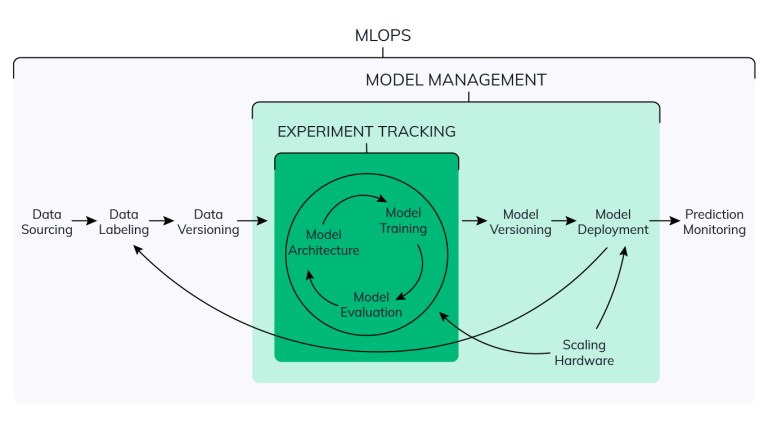
\includegraphics[width=.9\textwidth]{MLops.jpg} 
  \caption{MLops}
  \end{figure}

Dopo aver visto che tra i vari casi di studio troviamo una linea comune nella pipeline di utilizzo del Machine Learning, proviamo ad automatizzare le invarianti trovate nel capitolo precedente.\\
Negli ultimi anni i ricercatori stanno implementando diversi \Gls{framework} automatici che ci danno la possibilità di automatizzare il flusso di lavoro per la costruzione del modello.\\
Come visto in precedenza intendiamo: raccolta dati, creazione e implementazione del modello e successivamente alla distribuzione permettono la riproduzione e il monitoraggio.\\
Le pipeline ML, inoltre, aiutano a migliorare le prestazioni e la gestione dell'intero modello.\\
Possiamo semplicemente semplificare lo schema visto in precedenza come segue, lasciando la gestione del modello assegnata al \Gls{framework}.\\
Gli strumenti per l’orchestrazione ML sono usati per automatizzare e gestire i workflow e le infrastrutture delle pipeline con semplici interfacce, aiutando i data scientists e al team di ML di concentrarsi solo sul necessario.\\
Orchestrare un flusso di lavoro è fondamentale per un’azienda che investe nel ML, perciò è necessario capire come automatizzare il maggior numero di risorse, tra cui l’estrazione dell’output del modello con dei monitoraggi costanti durante la fase di produzione.\\
Questi campi che stiamo analizzando sono un sottoinsieme di MLOps: un insieme di pratiche per la collaborazione e la comunicazione tra data scientist e professionisti delle operazioni. Applicando queste tecniche pratiche aumenta la qualità finale, semplificando il processo di gestione e automatizza l’implementazione di modelli di ML e DL in ambienti di produzione su larga scala.(figura 4.1)


\section{\Gls{framework}}
  Prima di elencare una lista di tools di gestori di risorse di ML, diventa necessario anticipare una distinzione tra un software in fase di ricerca e un software giá a livello di produzione ovvero giá pronto per essere utilizzato a livello aziendale.\\
  Un software ancora in fase di ricerca, spesso utilizzato a livello accademico, offre delle funzionalitá magari non ancora rilasciate nel mondo ``Aziendale'' avendo delle "particolaritá" che altri software magari \textit{``in produzione''} non possiedono.\\
  Questi ultimi, a loro volta, si differenziano grazie a caratteristiche quali l'affidabilitá.\\
  Senza aver la pretesa di essere completi citiamo di seguito alcuni strumenti, giá rilasciati in produzione, piú conosciuti per l'orchestrazione di flussi di lavoro di apprendimento automatico.

  \newpage
  \subsection{ZenML} 
  ZenML è uno strumento open-source per operazione di ML.
  Lo strumento si focalizza sui problemi di riproduzioni basati sulla produzione, come le difficoltà di versioning e modelli, organizzazione di workflow di ML e la distribuzione. Può lavorare a fianco a un altro strumento di orchestrazione dei flussi di lavoro per fornire un semplice percorso per rilasciare il modello ML in produzione.\\
  È possibile verificare con precisione dati, modelli e configurazioni. Ti consente di valutare in maniera semi-automatica il modello, confrontare le pipeline di addestramento e distribuire la preelaborazione nel cloud.
  
\begin{figure}[htbp]
\centering
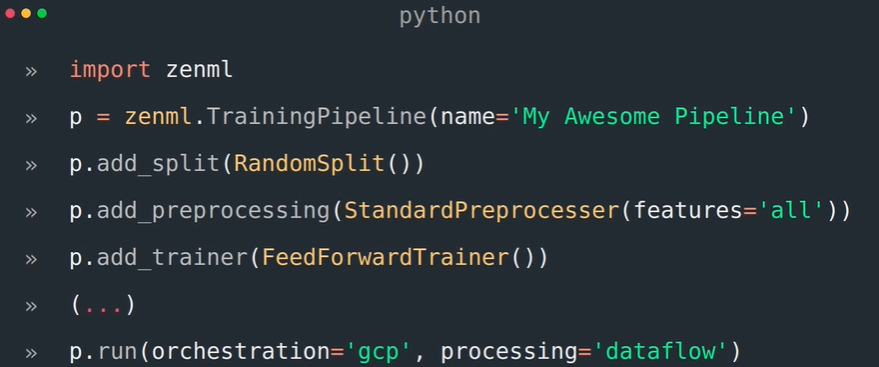
\includegraphics[width=.9\textwidth]{zenML.png} 
\caption{ZenML}
\end{figure}
  Come vediamo dalla figura 4.2 ogni metodo implementa uno specifico passaggio del workflow, vincolando i passaggi da eseguire sul modello a discrezione del \Gls{framework} stesso; se l'addestramento (\textit{add\textunderscore trainer}) appare prima del processamento dei dati (\textit{add\textunderscore preprocessing}), sará compito del framework nel metodo (\textit{run}) organizzare l'ordine delle operazioni da eseguire nel modello.
  
\subsection{Kedro}
  Kedro é uno strumento open-source di orchestrazione basato su Python, che permette di creare workflow per ML riproducibili, mantenibili e modulari, semplificando i processi e rendendoli più accurati.\\
  Kedro integra l’ingegneria del software in un ambiente di apprendimento automatico, con concetti quali: modularità, divisione degli interessi e versioning.\\
  Astraendo la pipeline, è possibile automatizzare le dipendenze tra il codice Python e la visualizzazione del Workflow; rendendo piu flessibile lo sviluppo di progetti di \textit{Data Science}.\\
  L’obiettivo principale è la creazione di codice di data science gestibile per affrontare le carenze di Jupiter(applicazione web open-source, utile per condividere documenti che contengono codice live, equazioni e grafi ecc.)\\
  Questo strumento crea un lavoro di squadra più semplice a vari livelli, e fornisce un efficiente ambiente di coding con codice modulare e riusabile.
\begin{figure}[htbp]
  \centering
  \includegraphics[width=.9\textwidth]{KedroPipeline.png} 
  \caption{Kedro}
  \end{figure}  
\subsection{Flyte}
\newglossaryentry{Kubernetes}{name={kubernetes},description={Sistema di open-source di orchestrazione e controllo di servizi containerizzati, uno dei modi ottimanali al giorno d'oggi per distribuire e eseguire applicazioni}}
  Flyte è uno strumento open-source di alta fascia che permette di facilitare la creazione di flussi di lavoro del ML. È una piattaforma di programmazione ad elaborazione distribuita e strutturata, con flussi di lavoro concorrenti, scalabili e mantenibili per l’apprendimento automatico e l’elaborazione dei dati.\\
  Flyte é scritto in Python ed é progettato per supportare flussi di lavoro ML complessi scritti in Python, Java e Scala.\\
  Flyte gestisce già più di dieci mila workflow, è basato su \Gls{Kubernetes} e offre portabilità, scalabilità e affidabilità.\\
  L’interfaccia è elastica, intuitiva e facile da usare; offre inoltre parametri, linee di dati e caching per organizzare i workflow.\\
  L’intera piattaforma è dinamica ed estensibile attraverso vari plug-in per assistere la creazione e l’implementazione dei vari workflow. Tali Workflow, a loro volta, possono essere reiterati, annullati, sperimentati e condivisi per accelerare il processo di sviluppo dell’intero team.\\
  Poiché ogni entità in Flyte è immutabile, insieme a ogni modifica esplicita assunta come nuova versione, diventa semplice ed efficiente iterare, sperimentare e tornare indietro nei Workflow.
\begin{figure}[htbp]
  \centering
  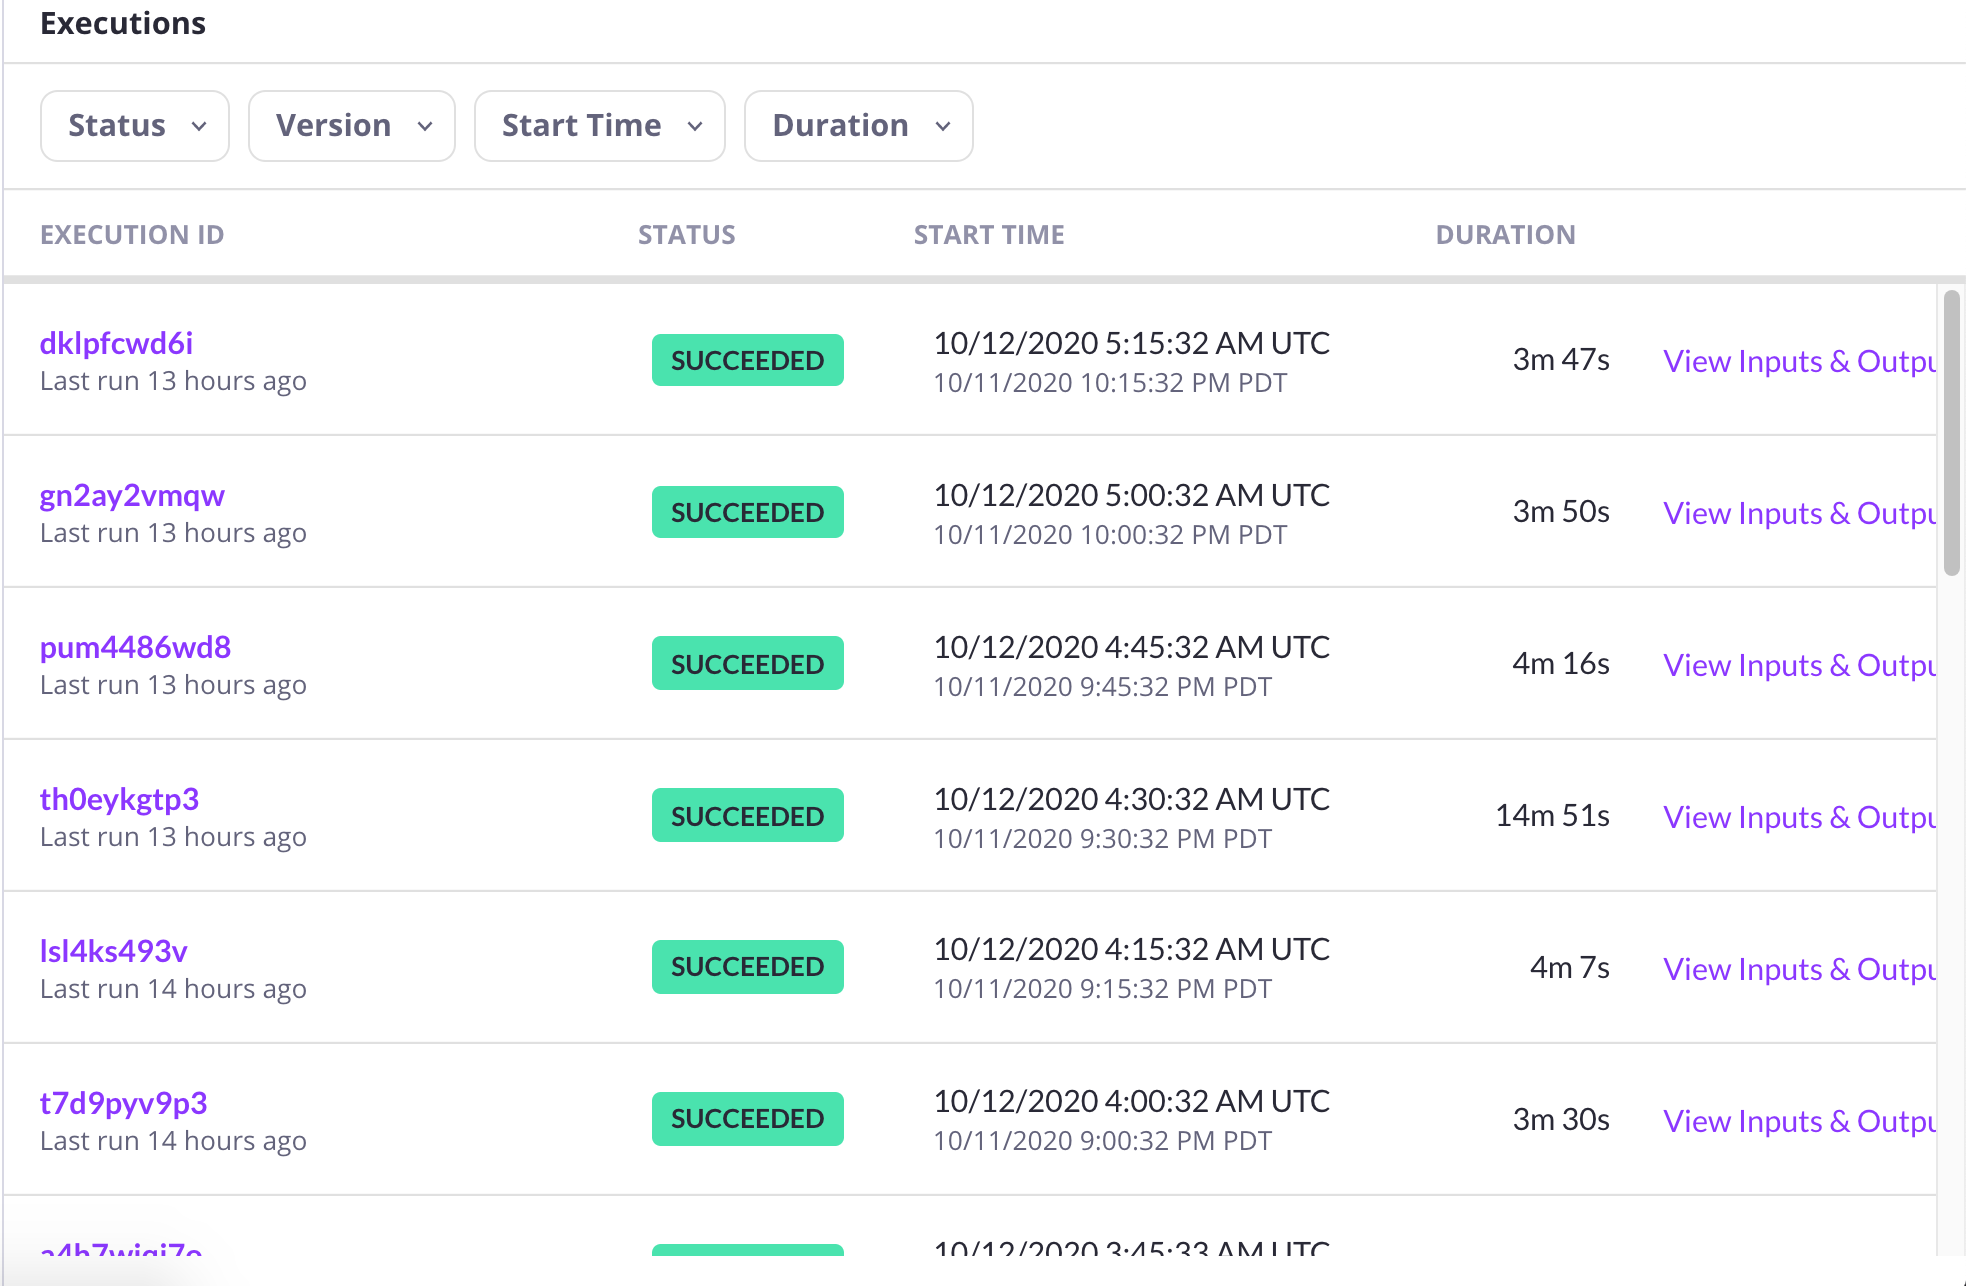
\includegraphics[width=.9\textwidth]{Flyte.png} 
  \caption{Flyte Console}
  \end{figure}

  \newglossaryentry{server-less}{name={server-less},description={Il ServerLess computing é un modello di sviluppo Cloud Native che consente agli sviluppatori di creare ed eseguire applicazioni senza gestire i server, i quali saranno astratti dallo sviluppo dell'app. La gestione delle risorse, la manutenzione e la scalabilitá del server saranno tutti compiti affidati al provider dei servizi cloud. }}
  \newglossaryentry{Microservizi}{name={microservizi},description={I Microservizi sono un approccio particolare alla realizzazione di applicazioni. Una applicazione diventa un insieme di servizi, i quali possono essere compilati e implementati in maniera indipendente. Inoltre ogni Microservizio puó funzionare, o meno, senza compromettere gli altri.}}
  \newglossaryentry{grafo aciclico}{name={grafo aciclico},description={Un grafo aciclico é un particolare tipo di grafo in cui non sono presenti cicli.}}
\newpage

\subsection{MLRun}
  MLRun è uno strumento open-source di orchestrazione di pipeline di ML. Offre un livello di astrazione per un'ampia varietà di stack tecnologici e consente a \textit{data engineer} e \textit{data scientist} di definire le funzionalità e i modelli, semplificando e accelerando il percorso verso la produzione.\\
  Esso integra un vasto reparto di strumenti e plugin per lavorare con caratteristiche e modelli insieme alla distribuzione del flusso di lavoro.\\
  MLRun dispone di un archivio di funzionalità e artefatti per controllare l’inserimento, l’elaborazione e l’archiviazione dei dati su più repository e con tecnologie diverse, rendendo possbile anche l'automatizzazione.\\
  È un elastico servizio ``\Gls{server-less}'' per convertire semplice codice in scalabili e organizzati ``\Gls{Microservizi}''; diventa così più semplice e leggero fare esperimenti, allenare i modelli e testarli, e implementare dei flussi di lavoro della pipeline in tempo reale.\\
  L’interfaccia utente complessiva ha una struttura centralizzata per gestire flussi di lavoro di ML. Le caratteristiche principali includono una rapida implementazione, elastica scalabilità, gestione delle funzionalità e un usabilità flessibile.\\
  \begin{figure}[htbp]
    \centering
    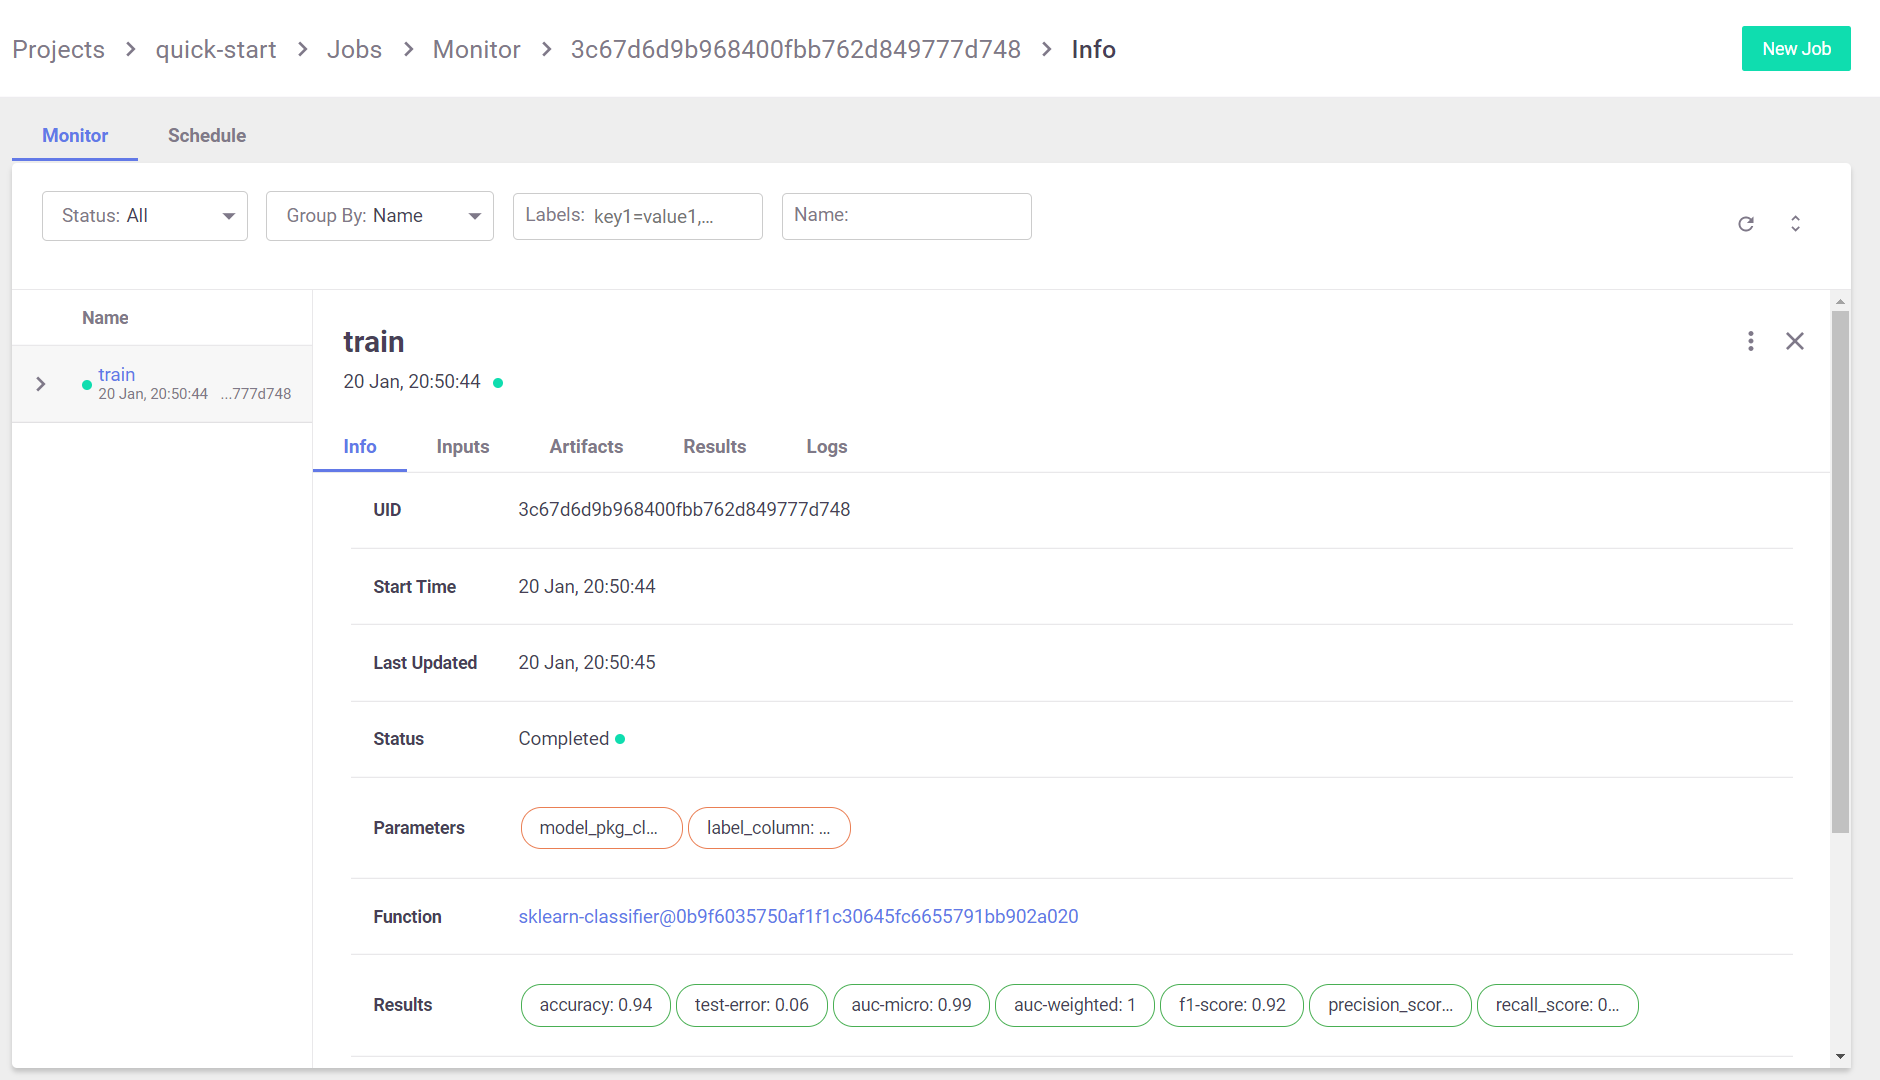
\includegraphics[width=.9\textwidth]{mlrun.png} 
    \caption{MLRun Console}
    \end{figure}

\section{Conclusioni}

Come spesso accade nel campo del \textit{Computer Science} uno stesso problema puó essere risolto attraverso l'utilizzo di diversi strumenti.\\
I framework che abbiamo selezionato sono open-source (tutti disponibili su \textit{github}) e forniscono tutti una  orchestrazione di flussi di lavoro per l'apprendimento automatico.\\
Kedro e Flyte sono i piú diffusi, tra cui Flyte, come citato nella sezione precedente, gestisce giá piú di 10 mila flussi di lavoro.
Ovviamente in base al caso di studio che prenderemo in considerazione si andrá a preferire un \Gls{framework} piuttosto che un'altro, a seconda delle caratteristiche che li differenziano, e che in parte abbiamo visto nella sezione precedente.\\
Ad esempio nel campo della radiologia, i medici si troverebbero in difficolta ad usare FW quali ZenML come libreria di Python come viceversa puó essere un approccio piú chiaro per sistemisti che lavorano nel campo del Networking, raccogliendo dati in real-time.\\
\Gls{framework} quali Flyte hanno un interfaccia intuitiva che magari permette anche a utenti che non lavorano costantemente nell'apprendimento automatico di fare predizione attraverso dei modelli.\\
Sia MLRun e Flyte sono estendibili attraverso diversi plug-in i quali possono diventare fondamentali qualora i dati in entrata sono di tipologie particolari(quali le immagini nel campo della radiologia o il Face2Face Traslation).\\
Nel campo dell'Intrusion Detection é necessario che ogni utente venga osservato \textit{concorrentemente} , questa possibilitá viene garantita da Flyte.
\end{document} 